\documentclass[letterpaper, 10pt, conference]{ieeeconf}  % Comment this line out if you need a4paper

%\documentclass[a4paper, 10pt, conference]{ieeeconf}% Use this line for a4 paper

\IEEEoverridecommandlockouts                              % This command is only needed if
                                                          % you want to use the \thanks command

\overrideIEEEmargins                                      % Needed to meet printer requirements.

%In case you encounter the following error:
%Error 1010 The PDF file may be corrupt (unable to open PDF file) OR
%Error 1000 An error occurred while parsing a contents stream. Unable to analyze the PDF file.
%This is a known problem with pdfLaTeX conversion filter. The file cannot be opened with acrobat reader
%Please use one of the alternatives below to circumvent this error by uncommenting one or the other
%\pdfobjcompresslevel=0
%\pdfminorversion=4

% See the \addtolength command later in the file to balance the column lengths
% on the last page of the document

% numbers option provides compact numerical references in the text.
% \usepackage{natbib}
\let\proof\relax
\let\endproof\relax
\usepackage{amsthm}
\usepackage{times}
\usepackage{multicol}
\usepackage[bookmarks=true]{hyperref}
\usepackage{xcolor}
\usepackage{hyperref}
\usepackage{amsmath, amssymb}
\usepackage{amsfonts}
\usepackage{graphicx}
\usepackage{siunitx}
\usepackage{standalone}
\usepackage{booktabs}
\usepackage[ruled,vlined,linesnumbered,noend]{algorithm2e}
\usepackage{mdframed}
\usepackage{fancyvrb,multirow}
\usepackage{soul}
\usepackage{dsfont,mathabx}
\usepackage{array, booktabs}
\usepackage{subfigure}
\usepackage{booktabs}
\usepackage{makecell}
\usepackage{threeparttable}



%%============================
%%============================

\newtheorem{theorem}{Theorem}
\newtheorem{proposition}{Proposition}
\newtheorem{lemma}[theorem]{Lemma}
\theoremstyle{definition}
\newtheorem{assumption}{Assumption}
\newtheorem{definition}{Definition}
\newtheorem{remark}{Remark}
\newtheorem{example}{Example}
\newtheorem{problem}{Problem}

% GENERAL
\newcommand{\todo}[1]{\textcolor{red}{TODO: #1}}
\newcommand{\improve}[1]{\textcolor{blue}{#1}}
\newcommand{\note}[1]{\textcolor{blue}{NOTE: #1}}
\newcommand{\question}[1]{\textcolor{orange}{Q: #1}}


%%%%%%%%%%%%%%%%%%%%%%%%%%%%%%%%%%%%%%%%%%%%%%%%%%%%%%%
%%%%


\title{\LARGE \bf
  PushAround: Collaborative Path Clearing via \\
  Physics-Informed Hybrid Search
}


% \author{Zili Tang$^1$, Zhongyuan Li$^1$,
%   Zhishao Qiao$^1$ and Meng Guo$^1$ %<-this % stops a space
%   \thanks{The authors are with: $^1$the College of Engineering,
%     Peking University, China;
%     This work was supported by the National Natural Science Foundation
%     of China (NSFC) under grants 62203017, T2121002, U2241214.
%     Contact: {\tt\small meng.guo@pku.edu.cn}.}% <-this % stops a space
% }

\begin{document}
\maketitle
\thispagestyle{empty}
\pagestyle{empty}


%%========================================


%%========================================
\begin{abstract}
The passage of large vehicles in cluttered environments is often blocked by
movable obstacles, motivating the use of mobile robot teams to proactively
clear traversable corridors. Existing approaches to Navigation Among Movable
Obstacles (NAMO) mainly plan abstract sequences of obstacle displacements but
neglect physical feasibility, overlooking robot dimensions, obstacle mass,
contact geometry, and required forces, which often leads to strategies that
fail in execution. This work introduces {PushAround}, a
physics-informed framework that guarantees feasible path clearing by coupling
geometric reasoning with dynamic validation. The core novelty is a hybrid
search that jointly determines which obstacles to displace and how to push
them, including contact points, directions, and forces. The framework builds a
W--Clearance Connectivity Graph (WCCG) to test vehicle passage, ranks frontier gaps to
prioritize obstacle-clearing actions, and incrementally expands feasible plans
by validating pushing modes. This integration ensures that solutions are both
geometrically valid and physically executable. Efficiency is achieved by
combining compact geometric reasoning with prioritized evaluation, avoiding
exhaustive simulation and improving scalability.
Extensive simulations and hardware experiments demonstrate robust success,
physical validity, and efficiency.
\end{abstract}

%%========================================
\section{Introduction}\label{sec:intro}
In many real-world scenarios, the path of a large vehicle or transport unit is obstructed by
movable obstacles such as pallets, boxes, or equipment, which motivates the use of a fleet of
mobile robots to actively clear traversable corridors and enable safe passage. This capability
is especially critical in unstructured or cluttered workspaces, including warehouses, disaster
sites, and crowded urban environments, where traditional path planning approaches assume
static obstacles and therefore fail to provide feasible solutions when direct paths are
blocked~\cite{liu2023path}. Research on Navigation Among Movable Obstacles (NAMO) has proposed strategies
for pushing, pulling, or rotating objects to create new routes~\cite{stilman2005navigation}, but these methods often
abstract away physical feasibility, ignoring key factors such as robot dimensions, obstacle
size and mass, contact geometry, applied forces, and the coupled dynamics of pushing. As a
result, the generated plans may be theoretically valid but physically unrealizable in practice.
This problem is particularly challenging because a single large robot is often unable to
independently clear a corridor; smaller robots are constrained by their limited size and reach,
making some obstacle boundaries inaccessible; and pushing actions introduce strong physical
coupling, where a single push may trigger chained motions of multiple obstacles, further
complicating prediction and planning.

\subsection{Related Work}\label{subsec:intro-related}
Navigation Among Movable Obstacles (NAMO) has been studied as a core
extension of motion planning in cluttered environments. Early approaches
planned sequences of obstacle displacements through pushing, pulling, or
rotating actions~\cite{stilman2005navigation}. Heuristic search methods improved scalability
by prioritizing which obstacles to move~\cite{stilman2007manipulation}, and graph- or
sampling-based algorithms enabled planning in larger workspaces~\cite{yao2024local}.
Multi-agent variants have also been explored~\cite{tang2024collaborative}. Despite these
advances, most NAMO approaches neglect physical feasibility, typically
treating robots as point agents with unlimited power and ignoring
dimensions, object mass, contact geometry, and force constraints. As a
result, many generated plans remain physically unrealizable~\cite{ren2025search}.

Collaborative pushing has also been investigated in the context of
multi-robot manipulation. Prior work has addressed synchronization of
forces~\cite{ni2023progressive}, stable contact maintenance~\cite{liu2025physics}, and cooperative
transport of objects in structured settings~\cite{ni2024physics}. These approaches
demonstrate effective coordination but generally focus on a single object
type and assume strict collision avoidance with surrounding obstacles.
Such assumptions exclude the possibility of exploiting inter-object
interactions, and the challenges of coupled dynamics and chain reactions
remain largely unaddressed~\cite{feng2025learning}.

Physics-informed planning has recently emerged to incorporate realistic
dynamics into motion planning. Some methods employ physics engines to
validate candidate manipulations~\cite{lin2019efficient} or simulate contact dynamics
during planning~\cite{rouxel2024multi}. While these works highlight the benefits of
embedding physics, they are mostly limited to single-object manipulation
or grasp planning. In addition, many approaches decouple abstract
planning from low-level physics checks~\cite{ni2023progressive}, which reduces efficiency,
and simulation-in-the-loop techniques face scalability challenges in
multi-robot, cluttered scenarios~\cite{feng2025learning}. A unified framework that
couples collaborative planning with physics-based feasibility for robust
path clearing has yet to be established.
%==============================
\subsection{Our Method}\label{subsec:intro-our}

This work introduces a physics-informed framework for collaborative multi-robot
pushing that actively constructs traversable corridors for large vehicles in
cluttered environments. The approach integrates three key components: a
W-Clearance Connectivity Graph (WCCG) to represent workspace connectivity under
vehicle width constraints and to identify blocking frontier gaps; a gap-ranking
strategy that estimates the cost of clearing each gap and prioritizes obstacles
for coordinated pushing; and a simulation-in-the-loop path construction scheme
that incrementally expands a configuration-space search tree and validates each
pushing mode through parallel physical simulation. This combination ensures that
planned actions account for robot dimensions, contact geometry, applied forces,
and chained obstacle motions, enabling physically feasible execution. The
framework is evaluated through extensive 2D and large-scale simulations as well
as hardware experiments, demonstrating robustness
under various dense obstacle configurations, and varying
team sizes.

The contributions of this work are twofold: (I) it presents the first unified
framework that couples multi-robot collaborative pushing with simulation-in-the-loop
planning to construct physically feasible paths in cluttered environments; (II)
it demonstrates significant improvements in feasibility, efficiency,
and scalability compared to existing NAMO and collaborative pushing approaches.

%%========================================
\section{Problem Description}\label{sec:problem}
%==============================================
\begin{figure*}[t!]
  \centering
  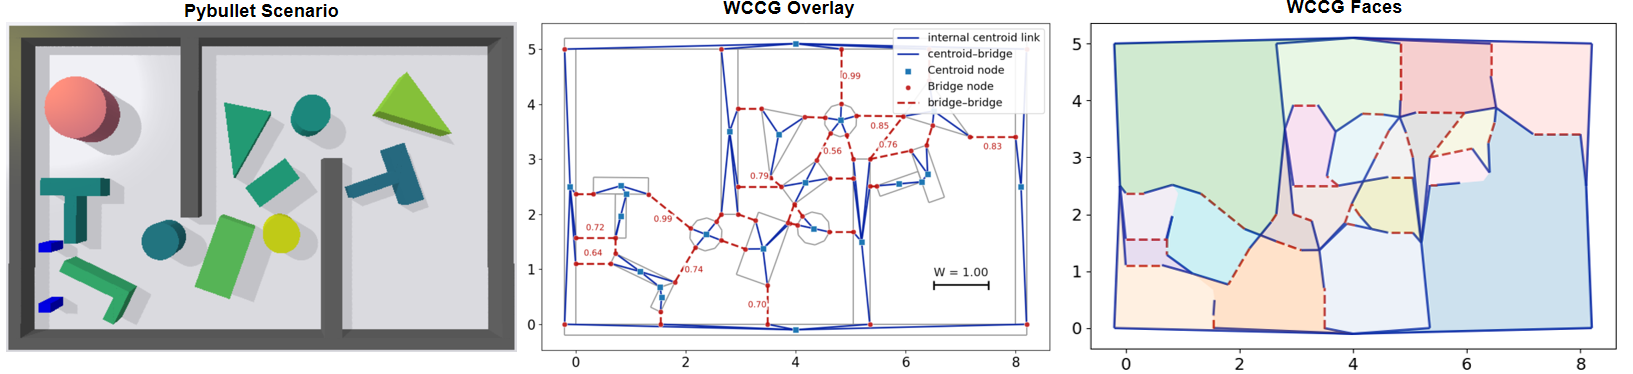
\includegraphics[width=0.95\linewidth]{figures/wccg.pdf}
  \vspace{-0.1in}
  \caption{Illustration of the W--Clearance Connectivity Graph (WCCG).
\textbf{Left:} Cluttered PyBullet scenario with the immovable walls and movable objects;
\textbf{Middle:} WCCG overlay with the centroid nodes (blue squares), bridge nodes
(red circles), centroid--bridge edges (blue), and bridge--bridge edges (red dashed)
annotated by the gap widths;
\textbf{Right:} Induced faces of the WCCG, where the colors indicate distinct connected
regions.}
  \label{fig:wccg}
  \vspace{-0.2in}
\end{figure*}
%==============================================
%==============================
\subsection{Workspace and Robots}\label{subsec:ws}
The workspace is a bounded planar region
$\mathcal{W}\subset\mathbb{R}^2$ that contains two types of
obstacles. A set $\mathcal{O}$ represents immovable structures,
while a set of $M$ movable rigid polygons is defined as
$\boldsymbol{\Omega}\triangleq\{\Omega_1,\cdots,\Omega_M\}\subset\mathcal{W}$.
Each movable obstacle $\Omega_m$ is characterized by its mass
$\mathsf{M}_m$, inertia $\mathsf{I}_m$, frictional parameters
(either identified or estimated), and state
$\mathbf{s}_m(t)\triangleq(\mathbf{x}_m(t),\psi_m(t))$,
where $\mathbf{x}_m(t)\in\mathbb{R}^2$ is the planar position of its centroid
and $\psi_m(t)\in\mathbb{R}$ its orientation angle. The region occupied by
$\Omega_m$ at time $t$ is denoted $\Omega_m(t)$.
Moreover, a small team of $N$ robots, indexed as
$\mathcal{R}\triangleq\{R_1,\cdots,R_N\}$, operates as a cooperative unit.
Each robot $R_i$ is modeled as a rigid body with state
$\mathbf{s}_{R_i}(t)\triangleq(\mathbf{x}_{R_i}(t),\psi_{R_i}(t))$,
where $\mathbf{x}_{R_i}(t)\in\mathbb{R}^2$ is its position and
$\psi_{R_i}(t)\in\mathbb{R}$ its orientation. The footprint of $R_i$ is
denoted $R_i(t)$. The instantaneous free space is given by:
\begin{equation}\label{eq:freespace}
\widehat{\mathcal{W}}(t)\triangleq\mathcal{W}\setminus\Big(
\mathcal{O}\cup\{\Omega_m(t)\}_{m=1}^{M}\cup\{R_i(t)\}_{i=1}^{N}
\Big),
\end{equation}
where $\widehat{\mathcal{W}}(t)$ excludes regions occupied by immovable
obstacles, movable obstacles, and robots.

%==============================
\subsection{External Vehicle and Clearance Goal}\label{subsec:vehicle}
An external vehicle $\texttt{V}$ of radius $W/2>0$ must navigate within the workspace
from a start configuration $\mathbf{s}_\texttt{V}^{\texttt{S}}$ to a goal configuration
$\mathbf{s}_\texttt{V}^{\texttt{G}}$. Since movable obstacles may obstruct the way, a
direct passage is not always feasible. Feasibility at time $t$ is captured by
the $W$-clearance condition
\begin{equation}\label{eq:wclear}
\exists\,\mathcal{P}^W_\texttt{V}\subset\widehat{\mathcal{W}}(t):\
\mathbf{s}_\texttt{V}^{\texttt{S}}\leadsto\mathbf{s}_\texttt{V}^{\texttt{G}},\;
\texttt{clr}(\mathcal{P}^W_\texttt{V})\ge W,
\end{equation}
where $\mathcal{P}^W_\texttt{V}$ is a continuous curve connecting start and goal inside
the free space, and $\texttt{clr}(\mathcal{P}^W_\texttt{V})$ denotes its minimum clearance
to surrounding obstacles.

%==============================
\subsection{Collaborative Pushing Modes}\label{ss:interaction_mode}
Thus, the robots may actively reconfigure $\boldsymbol{\Omega}$ by pushing obstacles.
The interaction with obstacle $\Omega_m$ is described by a pushing mode
$\boldsymbol{\xi}_m\triangleq(\mathcal{C}_m,\mathbf{u}_m)$,
where $\mathcal{C}_m\in(\partial\Omega_m)^N$ is the set of contact points
established by the robots, and $\mathbf{u}_m\in\mathbb{R}^{2N}$ encodes the body-frame forces
or an equivalent wrench profile. The admissible set of
modes is $\Xi_m$, determined by contact geometry and frictional limits.
Furthermore, the system evolution under a pushing mode
is captured by the transition operator below:
\begin{equation}\label{eq:transition}
  \mathbf{S}(t^+)\triangleq\Phi\big(\mathbf{S}(t),\,m,\,\boldsymbol{\xi}_m\big),
\end{equation}
where $\mathbf{S}(t)$ stacks all robot and obstacle states. The operator
$\Phi$ models the joint dynamics of robots and obstacles under contact. In
general, $\Phi$ is not available in closed form and is instead evaluated
through physics simulation.



%==============================
\subsection{Problem Statement}\label{subsec:objective}
The goal is to compute a hybrid schedule for the robots that reconfigures the movable
obstacles so that the vehicle admits a $W$-feasible path from start to goal.
The overall schedule for the robotic fleet is defined as:
\begin{equation}\label{eq:schedule}
\pi\triangleq\big\{(m_k,\boldsymbol{\xi}_k,\Delta t_k)\big\}_{k=1}^{K},
\end{equation}
where $\Omega_{m_k}\in \boldsymbol{\Omega}$ specifies the movable obstacle to manipulate,
$\boldsymbol{\xi}_k\in\Xi_{m_k}$ is the pushing mode, and
$\Delta t_k>0$ the duration of execution.
Thus, the optimization problem balances the execution time and the physical effort
of the clearance process, subject to various constraints, i.e.,
\begin{equation}\label{eq:problem}
\underset{\pi}{\textbf{min}}\ \Big{\{} T+\alpha\sum_{k=1}^{K}
J\!\left(m_k,\,\boldsymbol{\xi}_k,\,\mathbf{S}(\tau_k)\right)\Big{\}},
\end{equation}
where $T\triangleq\sum_{k=1}^{K}\Delta t_k$ is the total task duration,
$\alpha>0$ is a trade-off parameter, and $J(\cdot)$ is a simulation-based
control effort or feasibility cost evaluated at state $\mathbf{S}(\tau_k)$.
Note that the above optimization
problem is constrained by \eqref{eq:freespace}, \eqref{eq:wclear}, and
\eqref{eq:transition}, which jointly ensure collision-free evolution within
the workspace, valid dynamic transitions under pushing, and a terminal
$W$-clearance path for the vehicle.

% ==============================
\begin{remark}\label{remark:uniqueness}
  Problem~\eqref{eq:problem} above uniquely couples obstacle selection, pushing
  modes, and timing into a single hybrid optimization. This yields a
  combinatorial search space far more complex than classical NAMO, where
  prior work often assumes simple object shapes or hand-crafted contact
  modes~\cite{wang2006multi,goyal1989limit,chen2015occlusion,tang2023combinatorial}.
  \hfill $\blacksquare$
\end{remark}
% ==============================

%%========================================
% %% ========================================
\section{Proposed Solution}\label{sec:solution}

This section presents a unified framework for collaborative multi-robot pushing.
The approach consists of three main steps. First, a W-Clearance Connectivity Graph
(Sec.~\ref{subsec:wccg}) is constructed to test the existence of a path of width~$W$
and identify frontier gaps when blocked. Second, a gap-ranking strategy
(Sec.~\ref{subsec:gap}) estimates the cost of clearing candidate gaps and
guides robot coordination. Third, a simulation-in-the-loop search
(Sec.~\ref{subsec:simloop}) expands a configuration-space tree while validating
pushing actions through parallel physical simulation. The overall execution flow
and generalizations are summarized in Sec.~\ref{subsec:overall}.

% %% ========================================
%------------------------------
\begin{figure*}[t!]
  \centering
  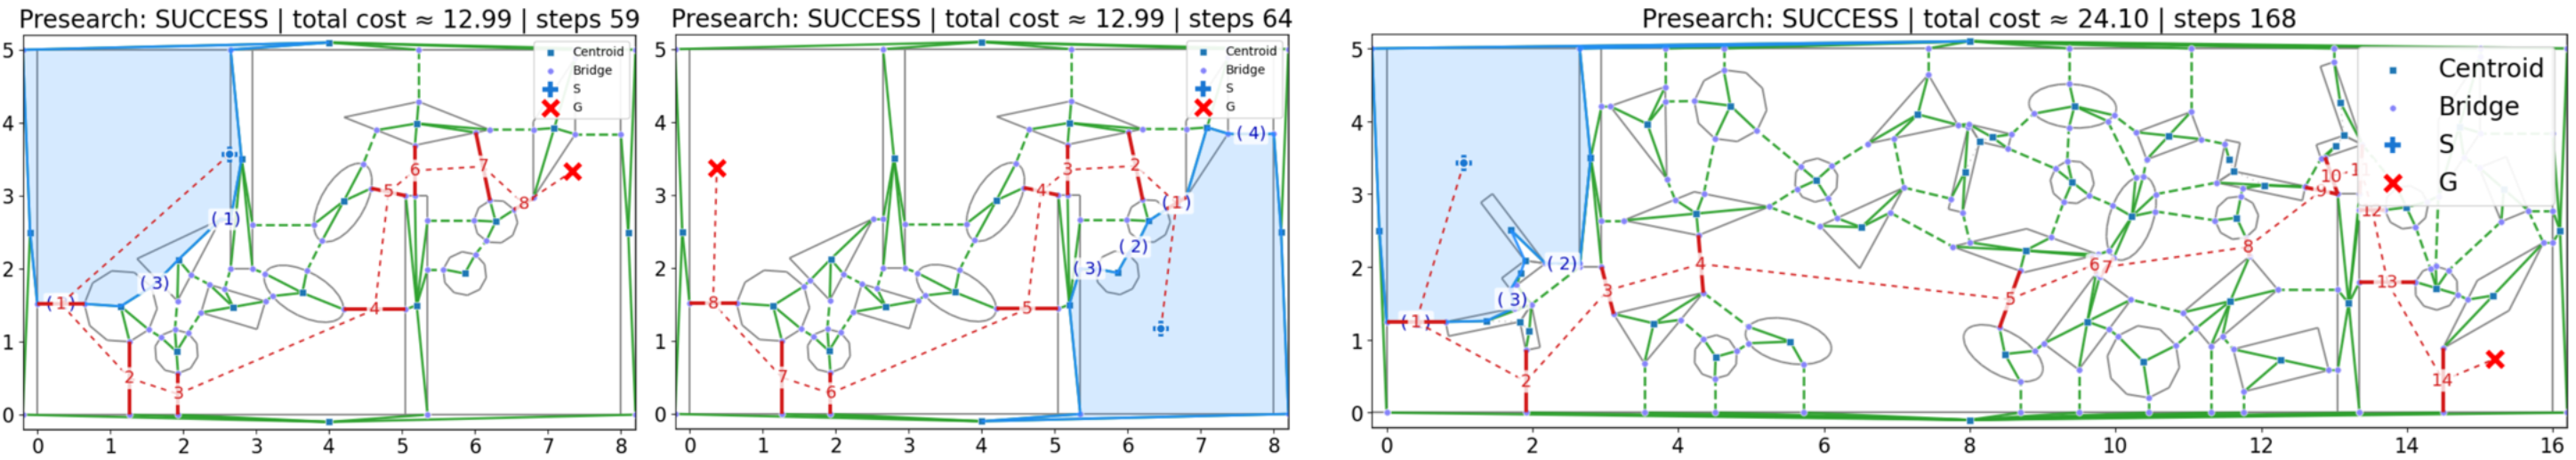
\includegraphics[width=0.95\linewidth]{figures/presearch.png}% or {presearch.pdf}
  \vspace{-0.15in}
\caption{
Illustration for {the ranking of potential gaps.}
Each panel shows the WCCG with the current face (light blue).
The algorithm (i) extracts the frontier loop from BugPlanner,
(ii) enumerates candidate bridge--bridge gaps on the loop,
(iii) assigns local first-hop ranks (blue numbers),
and (iv) simulates a short presearch to predict the full gap-crossing sequence (red numbers).
\textbf{Top}: start and goal swapped in the same map give symmetric
sequences with cost $12.99$;
\textbf{Right}: a larger map with about 30 obstacles produces a 14-gap sequence
with cost $24.10$.
}
  \label{fig:presearch}
   \vspace{-4mm}
\end{figure*}
%------------------------------
%==============================================
\subsection{W--Clearance Connectivity Graph}\label{subsec:wccg}

The feasibility of routing the vehicle reduces to whether a width-$W$ corridor 
connects $\mathbf{s}_\texttt{V}^{\texttt{S}}$ and $\mathbf{s}_\texttt{V}^{\texttt{G}}$. 
We introduce a W--Clearance Connectivity Graph (WCCG; Fig.~\ref{fig:wccg}) 
that encodes obstacle adjacencies under clearance $W$ and enables fast connectivity queries. 
Constructed directly from geometry (rather than grids/roadmaps), 
it avoids discretization error and remains consistent—crucial because connectivity is checked repeatedly 
during planning.

\subsubsection{Graph Construction}
The WCCG is built by decomposing each movable obstacle
$\Omega_m\in\boldsymbol{\Omega}$ into convex components. From each component
$C$, a centroid node $v_c$ is created. When two components $C_u$ and $C_v$
have closest points $p_u\in C_u$ and $p_v\in C_v$ with distance less than $W$, 
bridge nodes are added at $p_u$ and $p_v$. These bridge nodes are
connected by a bridge--bridge edge, annotated with the corresponding gap width
$w_{uv}\triangleq\|p_u-p_v\|$, and further linked back to their centroids with
centroid--bridge edges. Narrow passages with $w_{uv}<W$ are explicitly marked
as potential bottlenecks. The resulting graph is defined below:
\begin{equation}\label{eq:wccg}
\mathcal{G}_W\triangleq(\mathcal{V},\; \mathcal{E}_c\cup\mathcal{E}_b),
\end{equation}
where $\mathcal{V}$ contains all centroid and bridge nodes;
$\mathcal{E}_c$ is the set of centroid--bridge edges; and $\mathcal{E}_b$ the
set of bridge--bridge edges annotated by widths $w_{uv}$.

\subsubsection{Connectivity Criterion}\label{subsubsec:bugplanner}
Once $\mathcal{G}_W$ has been constructed, connectivity queries can be
performed without explicitly computing a geometric path. A frontier-tracing
procedure, similar to the BugPlanner~\cite{McGuireCroonTuyls2019}, starts from the vehicle start
$\mathbf{s}_\texttt{V}^{\texttt{S}}$, casts a ray toward the goal
$\mathbf{s}_\texttt{V}^{\texttt{G}}$, and explores the encountered loop of
frontier edges. If a valid exit is discovered, the process continues until the
goal is reached; otherwise a blocking cycle is returned. Successful execution
produces a skeleton $\Sigma$, which is an ordered sequence of centroid and
bridge nodes that certifies $\mathbf{s}_\texttt{V}^{\texttt{S}}$ and
$\mathbf{s}_\texttt{V}^{\texttt{G}}$ lie in the same connected face.
Let the $W$--clear free space be
$\mathcal{F}_W\triangleq\mathbb{R}^2\setminus(\mathcal{O}\oplus\mathbb{B}_{W/2})$,
where $\oplus$ denotes Minkowski addition and $\mathbb{B}_{W/2}$ is a closed
disk of radius $W/2$. A complete criterion for existence of a $W$--clear path
$\mathcal{P}^W_\texttt{V}$ is defined as:
\begin{equation}\label{eq:wccg_criterion}
\begin{aligned}
&\exists\,\mathcal{P}^W_\texttt{V}\subset\mathcal{F}_W:\
  \mathbf{s}_\texttt{V}^{\texttt{S}}\leadsto\mathbf{s}_\texttt{V}^{\texttt{G}} \Longleftrightarrow\
  \Big{\{}\mathbf{s}_\texttt{V}^{\texttt{S}},\mathbf{s}_\texttt{V}^{\texttt{G}}
  \ \text{belong to the} \\
  & \text{same face of }\mathcal{G}_W; \;\mathbb{B}_{W/2}(\mathbf{s}_\texttt{V}^{\texttt{S}}),
  \,\mathbb{B}_{W/2}(\mathbf{s}_\texttt{V}^{\texttt{G}})\subset\mathcal{F}_W\Big{\}},
\end{aligned}
\end{equation}
where $\mathbb{B}_{W/2}(\cdot)$ denotes a disk of radius $W/2$ centered at the
argument. This aligns with~\eqref{eq:wclear} for the external vehicle.

\subsubsection{Skeleton to Path}
The skeleton~$\Sigma$, the output of the previous step,
is an ordered sequence of centroid and bridge nodes connected by frontier
edges in $\mathcal{G}_W$. This skeleton serves as a compact certificate that
$\mathbf{s}_\texttt{V}^{\texttt{S}}$ and $\mathbf{s}_\texttt{V}^{\texttt{G}}$
lie in the same connected face. Given as input the skeleton $\Sigma$, together
with $\mathcal{G}_W$, the clearance $W$, and the endpoint disks
$\mathbb{B}_{W/2}(\mathbf{s}_\texttt{V}^{\texttt{S}})$ and
$\mathbb{B}_{W/2}(\mathbf{s}_\texttt{V}^{\texttt{G}})$, the output is an explicit
$W$--clear path $\mathcal{P}^W_\texttt{V}$. This path is constructed by sliding
each skeleton segment along the boundary of the inflated obstacles, offsetting
slightly inward into $\mathcal{F}_W$, and attaching short connectors inside the
endpoint disks. The resulting $\mathcal{P}^W_\texttt{V}$ remains in
$\mathcal{F}_W$, preserves the homotopy of $\Sigma$, and guarantees clearance of
at least $W$.


\begin{remark}\label{remark:wccg}
  The proposed WCCG differs from sampling- and grid-based planners in two key aspects:
  (I) It avoids discretization of $\mathcal{W}$ and is therefore free from
  resolution-induced errors;
  (II) It relies purely on geometry, which makes
queries highly efficient. These two features are crucial, since connectivity
checks and clearance tests are invoked many times within the hybrid
planner described in the sequel. \hfill$\blacksquare$
\end{remark}





%% \begin{algorithm}[t!]
%% \small
%% \caption{BugPlanner for $W$-width connectivity (skeleton witness)}
%% \label{alg:bugplanner}
%% \DontPrintSemicolon
%% \SetKwInOut{Input}{In}\SetKwInOut{Output}{Out}
%% \Input{$\mathbf{s}^{\texttt{S}}$, $\mathbf{s}^{\texttt{G}}$, WCCG}
%% \Output{if connected: skeleton $\Sigma$; else: frontier loop $\mathcal{L}$}
%% $P\leftarrow\mathbf{s}^{\texttt{S}}$, $\Sigma\leftarrow[\ ]$\;
%% \While{true}{
%%   \If{segment $P\mathbf{s}^{\texttt{G}}$ hits no edge}{\Return $\Sigma \cup \{\texttt{straight}(P,\mathbf{s}^{\texttt{G}})\}$}
%%   Build loop $\mathcal{L}$ by angle-follow from the hit edge; append traversed edges to $\Sigma$\;
%%   \If{$\mathrm{parity}(\mathcal{L},\,\mathbf{s}^{\texttt{S}}\mathbf{s}^{\texttt{G}})$ is odd}{\Return $(\emptyset,\mathcal{L})$}
%%   Choose exit $e$ on $\mathcal{L}$ (outward normal $\to\,\mathbf{s}^{\texttt{G}}$); append arc to $\Sigma$; $P\leftarrow e$ (tiny bias)\;
%% }
%% \end{algorithm}

% %% ========================================
%==============================================
\subsection{Ranking of Potential Blocking Gaps}\label{subsec:gap}

When the condition in~\eqref{eq:wccg_criterion} fails, the vehicle cannot
reach~$\mathbf{s}_\texttt{V}^{\texttt{G}}$ from
$\mathbf{s}_\texttt{V}^{\texttt{S}}$ through a $W$--clear path
$\mathcal{P}^W_\texttt{V}$. In this case, the planner must prioritize
\emph{blocking gaps} on the reachable frontier of $\mathcal{G}_W$. The goal of
this module is to provide an ordered list of such gaps, ranked by their
predicted cost to eventually yield a feasible path, which serves
as a critical guidance for the hybrid search in the sequel.

\subsubsection{Frontier Extraction and Candidate Gaps}
A BugPlanner query on $\mathcal{G}_W$, given
$(\mathbf{s}_\texttt{V}^{\texttt{S}},\mathbf{s}_\texttt{V}^{\texttt{G}},W)$,
either confirms connectivity or returns a counter--clockwise frontier loop
$\mathcal{L}$ that separates the two endpoints. The bridge--bridge edges
visible on $\mathcal{L}$ form the first--hop candidate set
$\Gamma_\mathcal{L}\triangleq\{g_1,\cdots,g_K\}$,
where each $g_k$ is a reachable candidate gap. These candidates are the inputs
to the ranking module, while the output will be an ordered list of the same
set sorted by predicted cost.

\subsubsection{Evaluation for Immediate Cost}
Each candidate $g\in\Gamma_\mathcal{L}$ is evaluated by combining the
cost for the robots to reach the gap and the effort required to widen it.
Let $\mathbf{s}_{\mathcal{R}}$ be the current robot positions,
and $\mathbf{o}_g$ as the outside insertion point of gap $g$. The
resulting one--hop cost is given by:
\begin{equation}\label{eq:step_cost}
\mathsf{C}\big(g \mid \mathcal{L}, \mathbf{s}_{\mathcal{R}}\big)
=\lambda_\texttt{t}\,\mathsf{C}_\texttt{t}\!\left(\mathbf{s}_{\mathcal{R}},\mathbf{o}_g\right)
+\lambda_\texttt{p}\,\mathsf{C}_\texttt{p}(g),
\end{equation}
where $\lambda_\texttt{t},\lambda_\texttt{p}>0$ are weighting factors
for the transition and pushing costs, respectively;
function $\mathsf{C}_\texttt{t}(\cdot)$ denotes the collision-free
distance between two points;
and the function~$\mathsf{C}_\texttt{p}(\cdot)$ measures the widening effort,
which increases when the gap is narrower than $W$,
or when the adjacent obstacles are heavier as scaled by the  mass of adjacent movable
obstacles.

%------------------------------
\begin{figure}[t!]
  \centering
  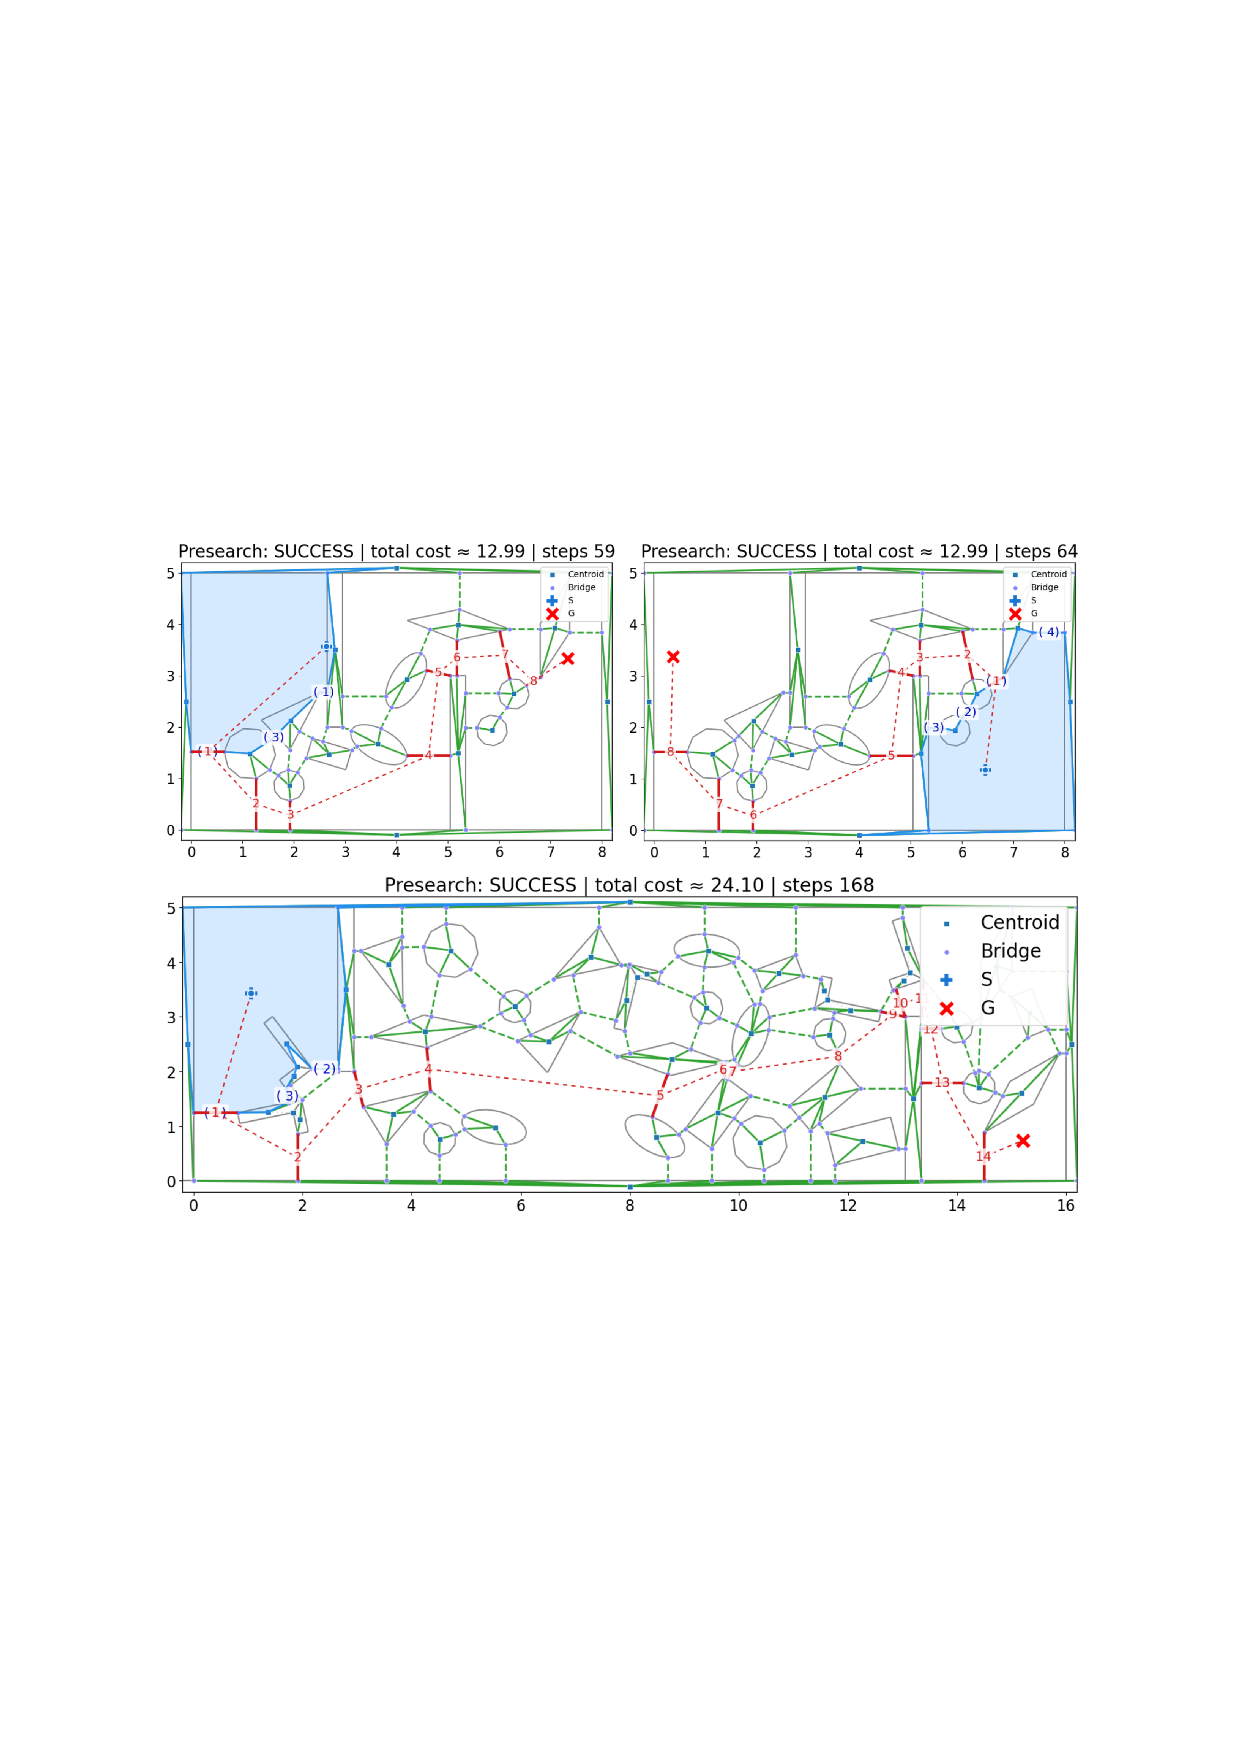
\includegraphics[width=\linewidth]{figures/presearch.pdf}% or {presearch.pdf}
  \vspace{-0.15in}
  \caption{
  Illustration for {the ranking of potential gaps.}
  Each panel overlays the WCCG together with the currently selected face (light blue).
  The algorithm (i) extracts the frontier loop from BugPlanner,
  (ii) enumerates candidate bridge--bridge gaps on the loop,
  (iii) assigns local first-hop ranks (blue numbers),
  and (iv) simulates a short presearch to predict the full gap-crossing sequence (red numbers).
  \textbf{Top:} identical environment with start and goal swapped;
  the resulting gap sequences are symmetric with identical predicted cost at $12.99$;
  \textbf{Bottom:} a larger map with about $30$ obstacles, where presearch returns a 14-gap sequence
  of predicted cost at $24.10$.
}

  \label{fig:presearch}
  \vspace{-0.1in}
\end{figure}
%------------------------------

\subsubsection{Long-term Cost w.r.t. Goal}
Furthermore, to prioritize gaps closer to the goal, a heuristic is added to the evaluation,
i.e.,
$h(g)=\eta\,\big\|\mathbf{o}(g)-\mathbf{s}_\texttt{V}^{\texttt{G}}\big\|$,
where $\eta>0$ is a scaling constant. Lastly, a short A$^\star$-style presearch virtually crosses
each candidate gap, recomputes the next frontier, and continues for a limited
beam width and depth. The predicted cost-to-connect is given by:
\begin{equation}\label{eq:pred_cost}
\widehat{\mathsf{Cost}}(g)\triangleq
\mathsf{C}\!\big(g \mid \mathcal{L},\mathbf{s}_{\mathcal{R}}\big)
+\!\!\!\sum_{g'\in\Pi^\star(g)}\!\!\!\big{\{}\mathsf{C}(g' \mid \cdot)+h(g')\big{\}},
\end{equation}
where $\Pi^\star(g)$ is the sequence of subsequent gaps discovered after
virtually crossing $g$;
the dots indicate updated inputs along that rollout;
and the scalar score $\widehat{\mathsf{Cost}}(g)>0$ for each candidate gap.
Consequently,
the final output of this module is the ranked list of candidate gaps, i.e.,
$\textsf{Rank}\big(\Gamma_\mathcal{L}\big)
\triangleq \textbf{argsort}_{g\in\Gamma_\mathcal{L}}\widehat{\mathsf{Cost}}(g)$,
which sorts $\Gamma_\mathcal{L}$ in ascending predicted cost. This
ordered set is passed to the hybrid search module, such that only the
promising gaps are expanded first.

\begin{remark}[Practical Improvement]\label{remark:gap}
Efficiency of the above ranking procedure can be improved by
caching frontier loops, storing the transitions
$(\mathcal{L},g)\mapsto\mathcal{L}'$, and accelerating the edge queries with
axis-aligned bounding-box culling. With a small beam width and depth
(typically around $8$), the runtime of ranking remains negligible compared to
the cost of simulation-based validation. \hfill$\blacksquare$
\end{remark}




%% %------------------------------
%% \begin{algorithm}[t]
%% \small
%% \caption{Frontier Presearch for Gap Ranking (compact)}
%% \label{alg:gap-ranking}
%% \DontPrintSemicolon
%% \SetKwInOut{Input}{In}\SetKwInOut{Output}{Out}
%% \Input{$\mathbf{s}^{\texttt{S}}$, $\mathbf{s}^{\texttt{G}}$, WCCG, $\lambda_{\mathrm{trans}}$, $\lambda_{\mathrm{push}}$}
%% \Output{First-hop gaps ranked by predicted cost}
%% $(\mathcal{L},\texttt{conn})\!\leftarrow\!\texttt{BugFrontier}(\mathbf{s}^{\texttt{S}},\mathbf{s}^{\texttt{G}})$;\;
%% \If{\texttt{conn}}{\Return $\emptyset$}
%% $\mathcal{C}\!\leftarrow$ bridge–bridge gaps on $\mathcal{L}$;\;
%% \For{$g\in\mathcal{C}$}{
%%   $J_1\!\leftarrow\!\lambda_{\mathrm{trans}}\mathsf{C}_{\mathrm{trans}}+\lambda_{\mathrm{push}}\kappa(g)[\max(0,W-w(g))+\delta]$;\;
%%   $(\texttt{succ},J_{\mathrm{tail}})\!\leftarrow\!\texttt{PresearchAfter}(g)$;\;
%%   $\widehat{\mathrm{Cost}}(g)\!\leftarrow\!J_1+\big(\texttt{succ}?J_{\mathrm{tail}}:\infty\big)$;\;
%% }
%% \Return $\mathrm{argsort}_{g\in\mathcal{C}}\widehat{\mathrm{Cost}}(g)$ (asc.)\;
%% \end{algorithm}

% %% ========================================
\begin{algorithm}[t]
\small
\caption{SiLS with Deferred Expansion (clean version)}
\label{alg:SiLS}
\DontPrintSemicolon
\SetKwInOut{Input}{In}\SetKwInOut{Output}{Out}
\SetKwFunction{Build}{BuildWCCG}
\SetKwFunction{Frontier}{BugPlannerFrontier}
\SetKwFunction{Rank}{PresearchRank}
\SetKwFunction{Predict}{SimPredict}
\SetKwFunction{Next}{NextBatch}

\Input{$\mathbf{s}^{\texttt{S}}$, $\mathbf{s}^{\texttt{G}}$, $W$, initial snapshot, batch size $B$}
\Output{Executable push plan or \texttt{fail}}

\BlankLine
\textbf{State of a node:} $\nu=(\texttt{snap}, \texttt{plan}, g, \mathcal{C}, j)$,
with candidates $\mathcal{C}$ (ranked) and cursor $j$.\;

\BlankLine
\textbf{Init:} $\nu_0\!\leftarrow\!(\texttt{snap}_0,\emptyset,0,\varnothing,0)$;\;
$\texttt{PQ}\!\leftarrow\!\{(\nu_0, f=\widehat{\mathsf{Cost}}_{\text{to-go}}(\texttt{snap}_0))\}$\;

\While{\texttt{PQ} not empty}{
  Pop $(\nu,f)$ with minimal $f$; \tcp*{$\nu=(\texttt{snap},\texttt{plan},g,\mathcal{C},j)$}
  \If{$\mathcal{C}=\varnothing$}{
    $(\texttt{connected}) \leftarrow \Build(\texttt{snap})$;\;
    \If{\texttt{connected}}{\Return \texttt{plan}}
    $\mathcal{L}\leftarrow \Frontier(\mathbf{s}^{\texttt{S}},\mathbf{s}^{\texttt{G}})$;\;
    $\mathcal{C}\leftarrow \Rank(\mathcal{L})$;\; $j\leftarrow 0$\;
  }
  $\mathcal{B}\leftarrow \Next(\mathcal{C}, j, B)$;\; $j\leftarrow j+|\mathcal{B}|$\;

  \ForEach{$\tau\in\mathcal{B}$ \textbf{in parallel}}{
    $(\texttt{ok}, \texttt{snap}', t_\text{push}) \leftarrow \Predict(\tau)$\;
    \If{\texttt{ok}}{
      $g' \leftarrow g + \mathsf{C}_{\mathrm{trans}} + t_\text{push}$;\;
      $h' \leftarrow \widehat{\mathsf{Cost}}_{\text{to-go}}(\texttt{snap}')$;\;
      Push $\big((\texttt{snap}',\,\texttt{plan}\!\cup\!\{\tau\},\,g',\,\varnothing,\,0),\, f'=g'+h'\big)$ into \texttt{PQ}\;
    }
  }
  \If{$j<|\mathcal{C}|$}{reinsert current $\nu$ into \texttt{PQ} with the same $f$}
}
\Return \texttt{fail}\;
\end{algorithm}


%==============================================
\subsection{Physics-Informed Hybrid Search}\label{subsec:simloop}

The hybrid search couples high-level decisions about blocking gaps with
low-level feasibility of multi-robot pushing. Unlike purely geometric
planners, this procedure simultaneously determines a sequence of gaps to clear
and physically feasible pushing actions, including directions, contact modes,
and forces. Parallel physics simulation is embedded so that many candidate
push strategies can be evaluated simultaneously at each expansion, and the resulting
successor states are returned to the search. This tight coupling of discrete
graph reasoning with continuous pushing dynamics is unique for the considered problem.

\subsubsection{Tree and Initialization}
The search tree $\mathcal{T}$ is composed of nodes
$\nu\triangleq(\mathbf{s},\pi)$, where $\mathbf{s}$ is the current system
state including the positions and orientations of all robots and movable
obstacles as in~\eqref{eq:transition}, and $\pi$ is the partial pushing
strategy realized so far as in~\eqref{eq:schedule}. Two global functions are
maintained: $\mathsf{Rank}(\nu)$ stores a ranked list of candidate gaps at this
node together with their exploration status, derived from~\eqref{eq:pred_cost};
and $\chi(\nu)$ returns the cumulative execution cost
from the root to $\nu$.
The root is initialized as
$\nu_0\triangleq(\mathbf{s}_0,\emptyset)$, where
$\mathbf{S}^{\texttt{S}}$ corresponds to the initial system state
$\mathbf{s}_0$. At initialization, $\chi(\nu_0)=0$, and
$\mathsf{Rank}(\nu_0)$ is constructed by first computing the frontier loop
$\mathcal{L}_\nu$ associated with~$\mathbf{s}_0$, then extracting the visible
gaps $\Gamma_{\mathcal{L}_\nu}$, and finally ranking them by their predicted
cost-to-connect.

\subsubsection{Node Selection}
At each iteration, the node with minimum best-first priority is selected from
the queue. The priority function balances the realized execution cost and the
estimated effort of remaining gaps:
\begin{equation}\label{eq:priority}
  f(\nu)\triangleq \chi(\nu)+\underset{g\in \textsf{Rank}(\nu)}{\textbf{min}}
  \widehat{\mathsf{Cost}}(g),
\end{equation}
where $\chi(\nu)$ is the cumulative execution cost so far, and the second term
is the minimum predicted remaining cost among the unexplored gaps of~$\nu$.
This scoring ensures that nodes are expanded in an order that jointly accounts
for physical effort already incurred and the most promising future actions.

\subsubsection{Node Expansion with Parallel Simulation}
When a node $\nu$ is selected for expansion, a batch of \emph{pushing
strategies} from $\mathsf{Rank}(\nu)$ is evaluated in parallel by simulation.
Each pushing strategy is defined as
\(\tau\triangleq(g,\mathbf{v},\boldsymbol{\xi})\), where
$g\in \boldsymbol{\Omega}$ is the chosen gap;
$\mathbf{v}\triangleq(v_x,v_y,\omega)\in \mathbb{R}^3$ is a short-horizon body
velocity for the manipulated obstacle;
and $\boldsymbol{\xi}\triangleq (\mathcal{C}_m,\mathbf{u}_m) \in (\partial\Omega_m)^N \times \mathbb{R}^{2N}$
is a contact mode specifying robot contact points and pushing forces as in~\eqref{eq:transition}.
Moreover, each candidate $\tau$ is first checked by a geometric quick-pass. If it passes,
it is evaluated by the simulator with the current state and pushing strategy:
\begin{equation}\label{eq:sim}
  (\mathbf{s}',\, \delta_\texttt{T},\, \delta_{\texttt{J}}) \triangleq \mathsf{EvalSim}
  \big{(}\nu,\, (g,\mathbf{v},\boldsymbol{\xi})\big{)},
\end{equation}
where $\mathbf{s}'$ is the successor state; $\delta_\texttt{T}>0$ is the time
cost; and $\delta_\texttt{J}$ is the control effort as in~\eqref{eq:problem}.
Thus, a successful evaluation produces a child
$\nu'\triangleq (\mathbf{s}',\pi')$, where $\pi'$ is obtained by appending
$\pi$ with $\tau$. The incremental realized cost of $\tau$ is
$\widehat{\mathsf{C}}(\nu,\,\tau)\triangleq \delta_\texttt{T} + \alpha\, \delta_\texttt{J}$,
with $\alpha>0$ the same trade-off parameter as in~\eqref{eq:problem}. The
cumulative cost is then updated by
$\chi(\nu')\triangleq \chi(\nu)+\widehat{\mathsf{C}}(\nu,\,\tau)$. Since many
pushing strategies are simulated concurrently, numerous successors can be
expanded in parallel at each iteration.

\subsubsection{Termination}
Termination occurs when a node $\nu$ reaches a state $\mathbf{s}$ for which a
$W$--clear path $\mathcal{P}^W_\texttt{V}$ exists from
$\mathbf{s}_\texttt{V}^{\texttt{S}}$ to $\mathbf{s}_\texttt{V}^{\texttt{G}}$,
as certified by~\eqref{eq:wccg_criterion}. In this case, the schedule $\pi$
stored in $\nu$ constitutes a complete solution to~\eqref{eq:problem}, encoding
both the sequence of gaps to clear and the physically feasible pushing actions
that realize them.

\begin{remark}[Parallel Expansion and Mode Reuse]\label{remark:simloop}
Efficiency of the hybrid search stems primarily from parallel evaluation of
pushing strategies, which allows many candidate futures to be simulated at once
for each expansion. Deferred expansion ensures that nodes with long candidate
lists remain in the priority queue until all tasks are attempted, preventing
search starvation. In addition, validated $(\boldsymbol{\xi},\mathbf{v})$ pairs
are cached locally within a subtree and stored in a persistent ModeTable for
reuse across similar obstacles, significantly reducing repeated physics calls.
These mechanisms yield orders-of-magnitude speedup relative to naive
simulation-based search. \hfill$\blacksquare$
\end{remark}

% %%========================================
%==============================
\subsection{Overall Analyses}\label{subsec:overall}


%==============================================
\subsubsection{Online Execution and Adaptation}\label{subsec:execute}

Once the hybrid pushing plan $\nu^\star$ is generated, the robot fleet executes the task
in real-time by following the guiding path $\overline{\mathbf{S}} = \{\mathbf{s}_0, \dots,
\mathbf{s}_L\}$. Each robot tracks the assigned trajectory segments, pushing the target
along the planned path while adjusting its motion based on the current target state
$\mathbf{s}_m(t)$ and interaction mode $\xi_n(t)$. The robots apply the desired forces
at the contact points $\mathbf{c}_n(t)$ using the control law:
\[
  \widehat{\mathbf{v}}_n = K_{\texttt{vel}} \left(\widehat{\mathbf{c}}_n - \mathbf{c}_n\right), \quad
  \widehat{\omega}_n = K_{\texttt{rot}} \left(\widehat{\psi}_n - \psi_n\right),
\]
to guide the object from the start to the goal while ensuring contact force consistency.
Transitioning between obstacles is handled according to the hybrid plan. Specifically,
as each robot pushes the object, it follows a **collision-free path** to the next set of
contact points on the next obstacle, ensuring that all movement respects the planned
interaction modes, and the sequence of obstacles is maintained. This transition is dynamically
adjusted as the robots continue pushing the target toward the goal.

In case of failures, such as when the object deviates from its expected position,
the algorithm triggers adaptation. If the object fails to reach the desired position,
the system checks the tracking error:
\[
  \mathrm{dist}(\mathbf{s}_m(t'), \varrho_\ell) \geq \delta_{\texttt{f}}, \quad
  \|\mathbf{s}_m(t') - \mathbf{s}_m(t'')\| < r_{\texttt{stuck}},
\]
and re-computes the entire hybrid plan based on the current system state. This includes
recalculating the sequence of movable obstacles to push, the contact points, and the
pushing forces to be applied. The updated plan is then executed with the control law in
\eqref{eq:control} to guide the robots toward the goal despite disruptions, ensuring
the task is completed even under unforeseen circumstances.



%==============================
\subsubsection{Complexity Analysis}\label{subsubsec:complexity}

The time complexity of the proposed method is dominated by three main components: the W-Clearance
Connectivity Graph (WCCG), gap-ranking strategy, and simulation-in-the-loop hybrid search. Constructing
the WCCG has a complexity of $\mathcal{O}(M^2 \log M)$, where $M$ is the number of movable obstacles,
due to the graph search and clearance checks. The gap-ranking strategy, which involves evaluating each
critical gap and ranking them based on their clearance and the obstacles’ mass, has a complexity of
$\mathcal{O}(G \log G + G M)$, where $G$ is the number of critical gaps and $M$ is the number of obstacles.
The most computationally intensive part is the simulation-in-the-loop hybrid search, which checks the feasibility
of each mode by simulating robot dynamics. The complexity for each simulation step is $\mathcal{O}(N^{3.5})$, where
$N$ is the number of robots, and the overall complexity of the hybrid search is $\mathcal{O}(N^{3.5} \cdot M \cdot L)$,
where $L$ is the number of keyframes in the path. Hence, the overall complexity is primarily determined by the hybrid
search algorithm.




%==============================
\subsubsection{Generalization}\label{subsec:general}

The proposed framework can be generalized in several directions. (I) \emph{Heterogeneous robots}:
When robots have varying capabilities, such as different maximum forces, the hybrid plan $\nu^\star$
should be adjusted by assigning more powerful robots to obstacles that require higher forces,
with smaller robots handling less demanding tasks. This adjustment is reflected in the interaction modes
$\boldsymbol{\xi} = (\mathbf{c}_1, \mathbf{f}_1, R_1), \dots, (\mathbf{c}_N, \mathbf{f}_N, R_N)$,
where $\mathbf{f}_n$ represents the force for each robot. (II) \emph{Simultaneous clearing}:
The framework can be extended to allow multiple obstacles to be pushed simultaneously,
improving the efficiency of path clearing. This requires modifying the WCCG, $\mathcal{G}^W(t)$,
to support parallel tasks and ensuring collision-free paths for multiple robots. (III) \emph{Dynamic
obstacle movement}: The method can handle dynamic obstacles by incorporating real-time sensor data
and updating the WCCG, allowing the hybrid search algorithm in Section~\ref{subsec:simloop} to adapt the plan
on-the-fly to avoid collisions and clear the path efficiently, even with moving obstacles.

% %%========================================

%%========================================
% ============================================================
\section{Numerical Experiments}
\label{sec:experiments}
We evaluate the proposed simulation-in-the-loop NAMO planner (SiLS)
in cluttered environments with both movable and immovable obstacles.
All components (W-CCG presearch, frontier extraction, and ModeTable prior)
are integrated as described in Sec.~\ref{sec:system}.
The implementation is in \texttt{Python~3} and simulations are run in
\texttt{PyBullet}~\cite{coumans2019} on a laptop with an Intel
Core i7\textendash1280P CPU. Videos and logs are provided in the
supplementary material.
\begin{figure}
  \centering
  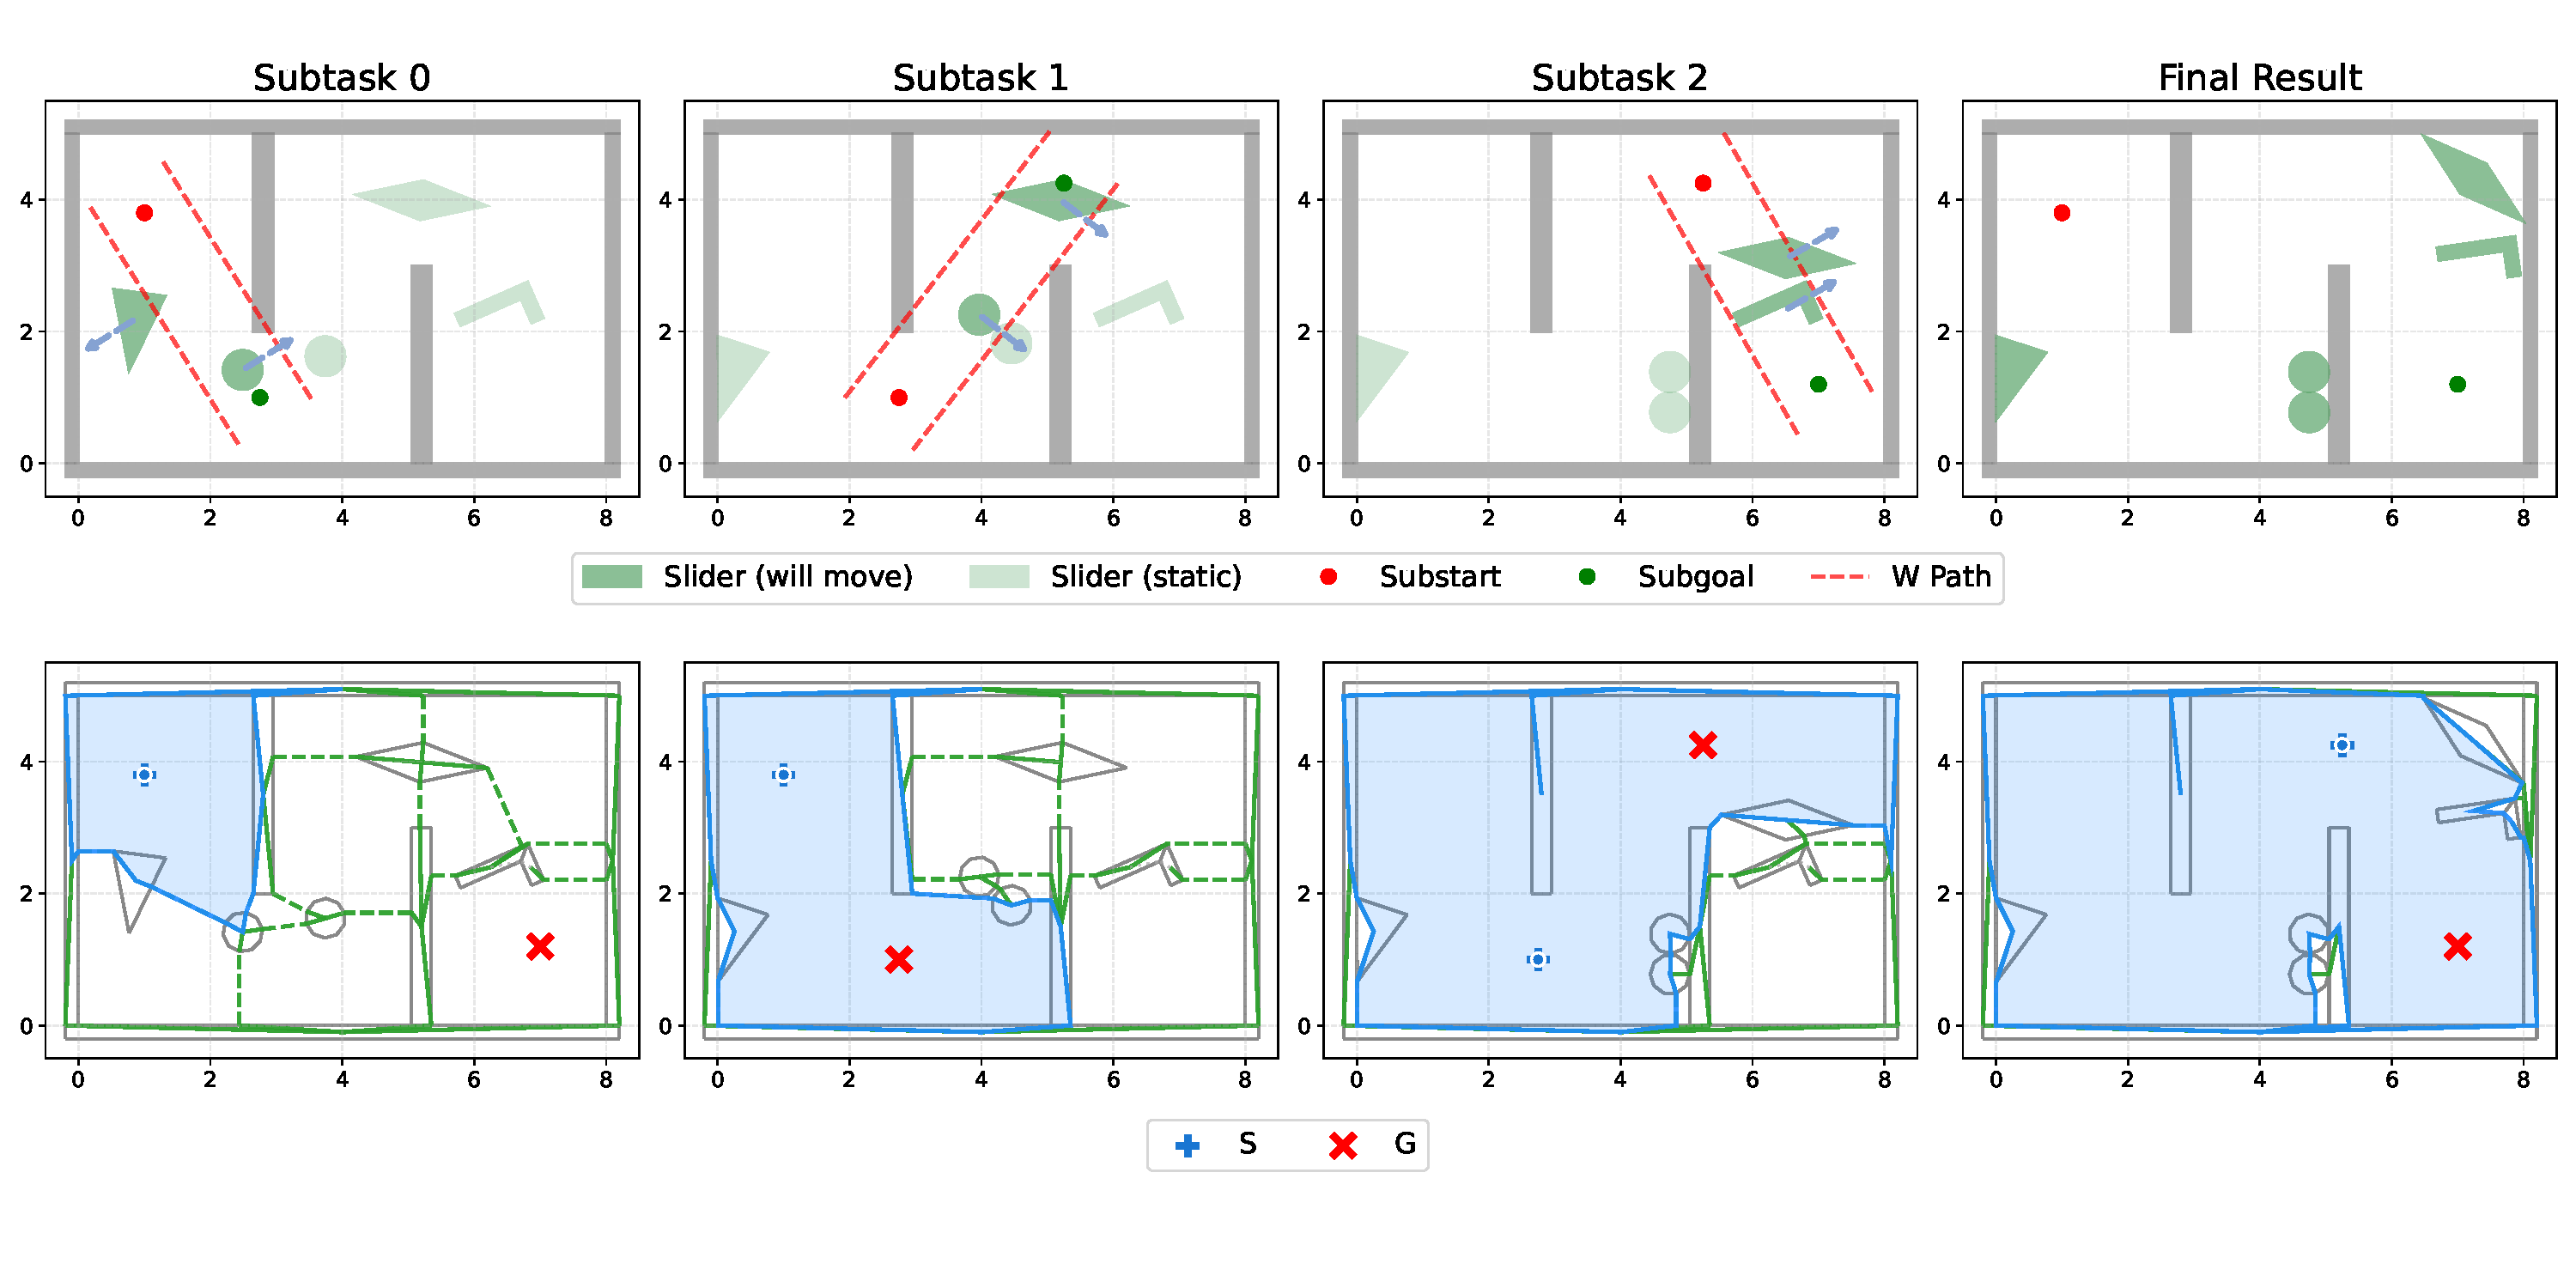
\includegraphics[width=\columnwidth]{figures/straight.pdf}

\caption{SL-Push}
\end{figure}

\begin{figure}
  \centering
  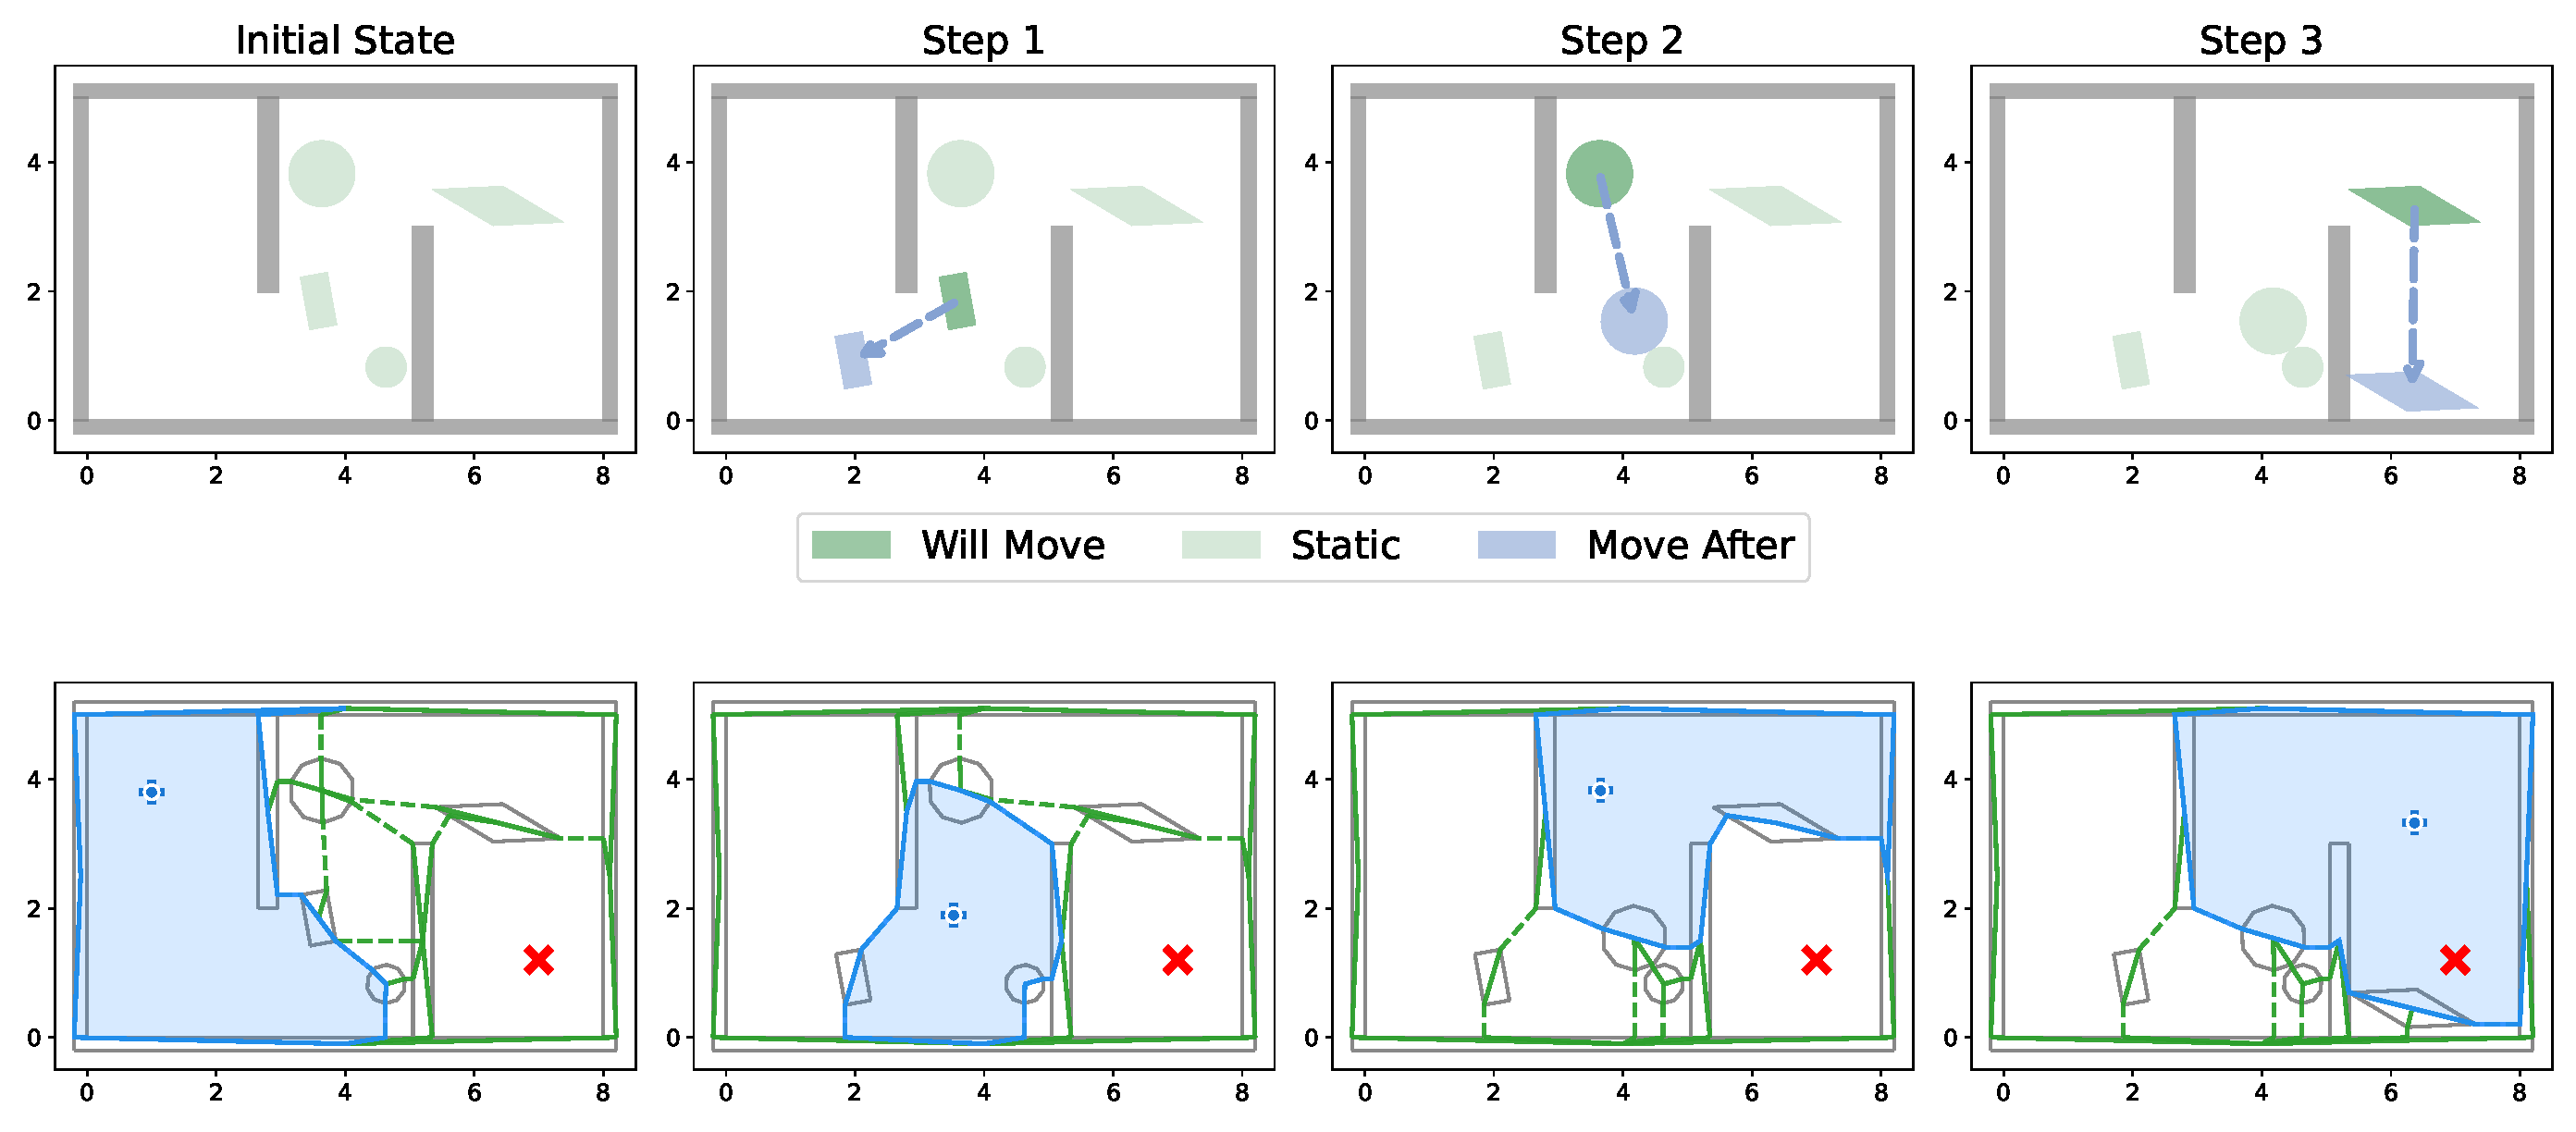
\includegraphics[width=\columnwidth]{figures/Recursive.pdf}
\caption{Rec-NAMO}
\end{figure}



% ========================================
\subsection{Numerical Simulations}
\label{subsec:sim}
% ========================================
\begin{figure}
  
\end{figure}
\subsubsection{\change{Setup}}
\label{subsec:sim-setup}
\change{
The physics step is $\Delta t = 1/120$\,s and the control period is
$1/40$\,s. Robots are disk/box pushers with risk radii consistent with
the $W$-clearance definition. Movable obstacles have masses uniformly
sampled in $[5,15]$\,kg; immovables are modeled with mass $0$.
A trial succeeds when a $W$-clear path from start to goal exists and the
target reaches its goal disc.
}

\paragraph{Workspace and scenarios.}
We use a \emph{nominal scenario} with an $8{\times}5$\,m bounded
workspace, two internal bars (bottlenecks), and a mixed pool of movable
shapes (curved and polygonal, including rings, ellipses, X/T/L/diamond,
arrow-like, rectangles, and cylinders). Two robots start in the lower
left; the target goal lies on the right side. Movables are randomly
placed with a minimum separation. We test \(10\text{--}15\) objects
over multiple seeds.

\paragraph{Geometry and caching.}
Collision checks use polygon/curve-edge models with convex
decomposition when needed. Ray--edge queries for frontiers are
vectorized with AABB culling. Frontier loops are cached by signatures and
transitions $(\mathcal{L},g)\!\mapsto\!\mathcal{L}'$ are memoized.

\subsubsection{\change{Algorithm Configuration}}
\label{subsec:algo-config}
\change{
Unless stated otherwise: per-task simulation horizon $=80$ steps,
up to $64$ candidate push tasks per expansion, and priority
$f = g + \widehat{\mathsf{Cost}}_{\text{to-go}}$ with heuristic factor $10$.
Gap sampling uses a softmax with temperature $0.05$.
ModeTable is enabled (auto-baked if missing).
A \emph{quick-pass} geometry screen may skip physics if a reference
rollout already clears the gap; otherwise a short-horizon simulation with
early stop is used. To avoid premature termination, a
\emph{deferred-reinsertion} rule keeps high-value but temporarily
unexpanded nodes in the queue and revisits them later.
}

\subsubsection{\change{Baselines}}
\label{subsec:baselines}
We compare against three representative families, all using the same
$W$-clearance criterion and contact models:

\begin{itemize}\itemsep2pt
  \item \textbf{DFS-WCCG:} Depth-first search over W-CCG adjacency with
  discrete axis-aligned pushes (object $\times$ \{$\leftarrow,\rightarrow,\uparrow,\downarrow$\}).
  \item \textbf{SL-Push:} Straight-line (or waypointed) route; blockers are
  cleared by (i) off-line minimal normal displacements or
  (ii) sim-in-the-loop normal pushes from near to far.
  \item \textbf{Rec-NAMO:} Recursive routing/pushing on a cost-weighted
  visibility graph: Dijkstra for routing, push-decomposition for local
  clearing; failures prune edges and replan.
\end{itemize}

\subsubsection{\change{Metrics}}
\label{subsec:metrics}
We report success rate, wall-clock time, number of node expansions,
number of simulated pushes, cumulative push time, average presearch
cost-to-go, quick-pass ratio, early-stop ratio, and worker-pool
utilization. Results are averaged over 10 seeds unless noted.

% ==============================
\subsubsection{Main Results}
\label{subsec:main-results}
Table~\ref{tab:main} summarizes performance on the nominal scenario.
SiLS attains higher success with fewer simulations and lower time due to:
(i) frontier-based gap ranking, (ii) ModeTable-guided push directions,
and (iii) quick-pass/early-stop. Deferred reinsertion prevents
priority-queue starvation by revisiting previously generated high-value
nodes when a batch of actions fails.

\begin{table}[t]
  \centering
  \begin{threeparttable}
  \caption{Performance on the nominal scenario with push-count (mean $\pm$ std).}
  \label{tab:main-push}
  \vspace{2pt}
  
  % 🔑 在这里调节列间距
  \setlength{\tabcolsep}{2.3pt} % 默认是 6pt,调小
  
  \begin{tabular}{lccccc}
  \toprule
  Method & Succ.~(\%) & \#PT (s) & \#ET (s) & \#Sims & \#Pushes \\
  \midrule
  DFS-WCCG            & 25 & -- & -- & -- & -- \\
  SL-Push (off-line)  & 62.5 & 0.02 & 145.147 & 0 & 7 \\
  SL-Push (sim)       & 75 & 25.09 & 246.825 & 16 & 8 \\
  Rec-NAMO            & 37.5 & 10.45 & 179.262 & 0 & 7 \\
  \textbf{SiLS (ours)}& \textbf{--} & \textbf{--} & \textbf{--} & \textbf{--} & \textbf{--} \\
  \bottomrule
  \end{tabular}
  
  \begin{tablenotes}[flushleft]\footnotesize
  \item \textbf{Metrics.} \emph{Succ.} = success rate; \emph{\#PT} = planning time; \emph{\#ET} = execution time;
  \emph{\#Sims} = simulations invoked; \emph{\#Pushes} = length of executed push sequence.
  \end{tablenotes}
  \end{threeparttable}
  \end{table}
  


\subsubsection{Ablations}
\label{subsec:ablations}
We remove one component at a time: (i) W-CCG presearch (random gap order),
(ii) ModeTable prior (fallback “away\,+\,jitter” only),
(iii) quick-pass/early-stop (always full physics),
(iv) deferred reinsertion (terminate on empty queue).
Table~\ref{tab:ablation} shows consistent drops in success and increased
time/\#Sims when any component is disabled.

\begin{table}[t]
  \centering
  \caption{Ablations on the nominal scenario (fill with measurements).}
  \label{tab:ablation}
  \vspace{2pt}
  
  % 🔑 调整列间距和行距(只对本表生效)
  {%
  \setlength{\tabcolsep}{3pt} % 列间距缩小
  \renewcommand{\arraystretch}{0.9} % 行距缩小
  
  \begin{tabular}{lcccc}
  \toprule
  Variant & Succ.~(\%) & Time (s) & \#Sims & Quick-pass (\%) \\
  \midrule
  SiLS (full)            & -- & -- & -- & -- \\
  \ \ w/o presearch      & -- & -- & -- & -- \\
  \ \ w/o ModeTable      & -- & -- & -- & -- \\
  \ \ w/o quick-pass/ES  & -- & -- & -- & -- \\
  \ \ w/o reinsertion    & -- & -- & -- & -- \\
  \bottomrule
  \end{tabular}
  }% 局部作用域结束
  
  \end{table}
  

\subsubsection{Efficiency and Scalability}
\label{subsec:eff}
\textbf{Frontier caching} makes BugPlanner near-linear in visible edges.
\textbf{Parallel prediction} uses a persistent worker pool with per-round
broadcast of snapshots and reachable-contact sets to reduce IPC.
\textbf{Quick-pass} and \textbf{early-stop} skip or truncate physics when
geometry suffices. \textbf{Deferred reinsertion} maintains steady depth
growth even when many pushes are rejected.

\subsubsection{Qualitative Results}
\label{subsec:qual}
Figure~\ref{fig:qual} shows a typical run: frontiers and ranked gaps,
a top-ranked gap sequence, simulated pushes that widen bottlenecks, and
the final $W$-clearance path. Per-step overlays and GIFs are produced by
a lightweight snapshot logger.

% \begin{figure}[t]
% \centering
% \includegraphics[width=0.98\linewidth]{figures/qual_demo.pdf}
% \caption{Representative run: frontier (blue), ranked gaps (color-coded by
% predicted cost), simulated pushes (red), and the resulting
% $W$-clearance path (green).}
% \label{fig:qual}
% \end{figure}

\subsubsection{Reproducibility}
\label{subsec:repro}
Random seeds are fixed, JSONL snapshots are logged, and the driver and
scenario generator are released. ModeTable entries are auto-generated if
absent to ensure repeatability across machines.


%%========================================
\section{Conclusion} \label{sec:conclusion}
This work introduces a multi-robot approach for path clearing in unstructured environments, utilizing
a hybrid search algorithm to plan and execute the sequence of obstacles, contact points, and forces efficiently.
The framework demonstrates real-time adaptability to dynamic scenarios. Future work will address uncertainties
such as estimating obstacle positions without external monitoring, handling uncertain obstacle masses, and managing
partial robot visibility to improve robustness and performance in real-world, dynamic environments.

%%========================================

\newpage
%========================================
\bibliographystyle{IEEEtran}
\bibliography{contents/references}

\end{document}
